\documentclass[11pt]{article}
\textwidth 15.9cm
\textheight 23. cm
\addtolength{\oddsidemargin}{-11.5mm}
\addtolength{\evensidemargin}{-11.5mm}
\addtolength{\topmargin}{-19.0mm}

% \usepackage{amsmath}
\usepackage{amsmath,amssymb}
\usepackage[ansinew]{inputenc}
\usepackage[bbgreekl]{mathbbol}
\usepackage{stmaryrd}
\usepackage{bm}

\usepackage{newtxtext,newtxmath}

\usepackage{graphicx}
\usepackage{hyperref}
\usepackage{url}
\usepackage[numbers,square]{natbib}
\usepackage{multirow}
\usepackage{tikz}
\usepackage{tikz-cd}
\usetikzlibrary{arrows,matrix}
\usepackage{bbm}
\usepackage{authblk}
\usepackage{subcaption}
\renewcommand{\Affilfont}{\footnotesize}
%\renewcommand{\Authfont}{\normalsize}

\usepackage{stmaryrd}
\usepackage{comment}
\usepackage{showlabels}
\usepackage{soul}
%\usepackage[dvipsnames]{xcolor}

\usetikzlibrary{calc,patterns,shapes.geometric}
\usetikzlibrary{arrows,shapes,positioning}
\usetikzlibrary{decorations.markings,decorations.pathmorphing,decorations.pathreplacing}
\usetikzlibrary{decorations.text,decorations.shapes}

%%%%%%%% MACROS
\input{gempic_spectral_macros}

\newcommand{\hi}{\hat{i}}
\newcommand{\hj}{\hat{j}}
\newcommand{\hk}{\hat{k}}

% \newcommand{\arr}[1]{{\bs{\mathsf{#1}}}}

% matrices
\newcommand{\hodgeZero}{\mathbb{H}_0}
\newcommand{\hodgeOne}{\mathbb{H}_1}
\newcommand{\hodgeTwo}{\mathbb{H}_2}
\newcommand{\hodgeThree}{\mathbb{H}_3}
\newcommand{\hodgeDualZero}{\tilde{\mathbb{H}}_0}
\newcommand{\hodgeDualOne}{\tilde{\mathbb{H}}_1}
\newcommand{\hodgeDualTwo}{\tilde{\mathbb{H}}_2}
\newcommand{\hodgeDualThree}{\tilde{\mathbb{H}}_3}
\newcommand{\hodgeDualZeroB}{\mathbb{H}^*_0}
\newcommand{\hodgeDualOneB}{\mathbb{H}^*_1}
\newcommand{\hodgeDualTwoB}{\mathbb{H}^*_2}
\newcommand{\hodgeDualThreeB}{\mathbb{H}^*_3}

\newtheorem{theorem}{Theorem}
\newtheorem{lemma}{Lemma}
\newtheorem{remark}{Remark}
\newtheorem{definition}{Definition}
\newtheorem{assumption}{Assumption}



\title{Notation conventions in GEMPIC}


\author[1]{The Gempic development team}
\affil[1]{Max-Planck-Institut f\"ur Plasmaphysik, Garching, Germany}



\begin{document}


\maketitle

\begin{abstract}
This note describes some conventions that should be followed in the GEMPIC code
and its documentation.
\end{abstract}

\tableofcontents

\section{Solving Maxwell's equations with discrete differential forms}
\label{sec:Maxwell_with_discrete_forms}

\subsection{Continuous and discrete Maxwell equations}
\label{sec:maxwell_cont_discrete}

In GEMPIC, Maxwell's equations 
\begin{equation} \label{eq:maxwell}
	\left\{\begin{aligned}	
		&\partial_t {\bs D} - \curl {\bs H} = -{\bs J}
		\\
		&\partial_t {\bs B} + \curl {\bs E} = 0
	\end{aligned}\right.
	\qquad \qquad
	\left\{\begin{aligned}	
		&\Div {\bs D} = \rho
		\\
		&\Div {\bs B} = 0
	\end{aligned}\right.
\end{equation}
are discretized in space by matrix equations of the form
\begin{equation} \label{eq:max_mat}
	\left\{\begin{aligned}	
		&\partial_t \tildearr{D} - \tildemat{C} \tildearr{H} = -\tildearr{J}
		\\
		&\partial_t \arr{B} + \mat{C} \arr{E} = 0
	\end{aligned}\right. 
	\qquad \qquad
	\left\{\begin{aligned}	
		&\tildemat{D} \tildearr{D} = \tildearr{\rho} 
		\\
		&\mat{D} \arr{B} = 0
	\end{aligned}\right.	
\end{equation}
where the unknowns are arrays of geometric freedom representing 
the discrete fields and densities, while $\mat{C}$ and $\mat{D}$
(resp. $\tilde{\mat{C}}$ and $\tilde{\mat{D}}$)
are matrices representing the curl and div operators on a primal 
(resp. dual) Cartesian grid. 

At the continuous level, Maxwell's equations are completed with constitutive 
relations of the form
\begin{equation} \label{eq:const}
\left\{\begin{aligned}
	&{\bs H} = \cH_\mu {\bs B}
	\\
	&{\bs E} = \cH_\ve {\bs D}
\end{aligned}\right.
\end{equation}
where $\cH_\mu$ and $\cH_\ve$ are continuous Hodge operators
associated with the magnetic and electric permittivity tensors.
For constant permittivities in $\RR^3$ these are simply (scaled) identity operators.
At the discrete level, \eqref{eq:const} becomes
\begin{equation} \label{eq:const_mat}
	\left\{\begin{aligned}
		&\tilde {\arr{H}} = \mat{H}_2 \arr{B}
		\\
		&\arr{E} = \tilde {\mat{H}}_2 \tilde {\arr{D} }
	\end{aligned}\right.
\end{equation}
where $\mat{H}_2$ and $\tilde{\mat{H}}_2$ are Hodge matrices approximating 
the continuous Hodge operators.

Finally we note that an electrostatic field of the form 
$$
\bE = -\grad \phi
$$
may be discretized as a discrete gradient:
$$
\arr{E} = -\mat{G} \arr{\phi}.
$$



\subsection{Continuous and discrete de Rham sequences}
\label{sec:deRham_cont_discrete}

Together with their natural differential operators,
the spaces containing the continuous and discrete solutions of the above equations
form a series of de Rham sequences which in 3D can be gathered in the following diagram:
\begin{figure}
	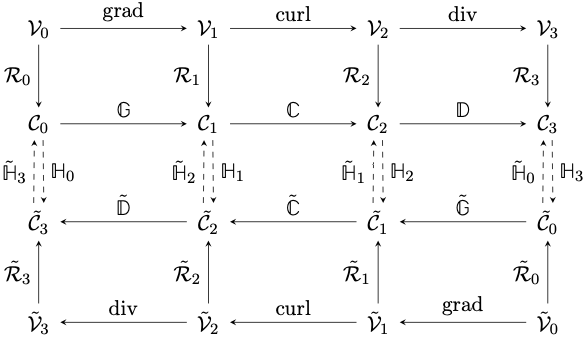
\includegraphics[width=130mm]{deRhamCGL.png}
	\caption{3D de Rham diagram}% Captions are necessary for references to work
	\label{fig:CGL}
\end{figure}
Here the first and last rows are sequences of continuous spaces
$\mathcal{V}_\ell$ and $\tilde{\mathcal{V}}_\ell$,
while the middle rows are to sequences of discrete spaces 
$\mathcal{C}_\ell$ and $\tilde{\mathcal{C}}_\ell$: 
in GEMPIC these are spaces of coefficients corresponding to geometric degrees of freedom, 
defined on the primal and dual grids (see below).

Moreover, the first two rows correspond to the primal de Rham sequences,
while the last two rows correspond to the dual de Rham sequences:
the Hodge matrices $\mathbb{H}^\ell$ (resp. $\tilde{\mathbb{H}}^\ell$) 
allow to map the primal (resp. dual) discrete spaces to their dual 
(resp. primal) counterparts, leading to the discrete constitutive relations \eqref{eq:const_mat}.

More details on these spaces are given below. We also refer to e.g. 
\cite[Sec.~3]{Arnold.Falk.Winther.2010.bams} 
for a description of these sequences in terms of Hilbert complexes 
and discretization with Finite Element (FEEC) spaces.

In GEMPIC we consider
\begin{equation} \label{eq:EBHD}
	\arr{\phi} \in \mathcal{C}_0, 
	\quad 
	\arr{E} \in \mathcal{C}_1, 
	\quad
	\arr{B} \in \mathcal{C}_2, 
	\quad
	\tilde{\arr{H}} \in \tilde{\mathcal{C}}_1, 
	\quad
	\tilde{\arr{D}} \in \tilde{\mathcal{C}}_2
	\quad
	\tilde{\arr{J}} \in \tilde{\mathcal{C}}_2, 
	\quad
	\tilde{\arr{\rho}} \in \tilde{\mathcal{C}}_3
\end{equation}
which corresponds to characterizing the discrete fields and densities as arrays of 
geometrical degrees of freedom.

\subsection{Geometrical degrees of freedom and reduction operators}
\label{sec:dofs_and_reductions}

The coefficients of the discrete fields and densities correspond to geometric
degrees of freedom, such as node values, edge, face or cell integrals
on the primal grid (with nodes denoted with integer indices) or on the 
dual one (with nodes denoted with half-integer indices).

% \begin{tikzpicture}
% 	% primal grid with bullets
% 	\draw (0,0) grid (4,4);
%     \foreach \x in {0,1,2,3,4}
%     \foreach \y in {0,1,2,3,4}
%     \node at (\x,\y) {$\bullet$};   

% 	% dual grid with half-integer offset in dashed lines
% 	\draw[step=1, dashed, xshift=0.5cm, yshift=0.5cm] (-0.5,-0.5) grid (3.5,3.5);

%     % label coordinates as x_i on the x axis
%     \foreach \x/\y in {0/-.5,1/-.5,2/-.5,3/-.5,4/-.5}
%     \node at (\x,\y) {$x_\x$};

%     % label coordinates as y_i on the y axis
%     \foreach \x/\y in {-.5/0, -.5/1, -.5/2, -.5/3, -.5/4}
%     \node at (\x,\y) {$y_\y$};

% \end{tikzpicture}
\begin{figure}
	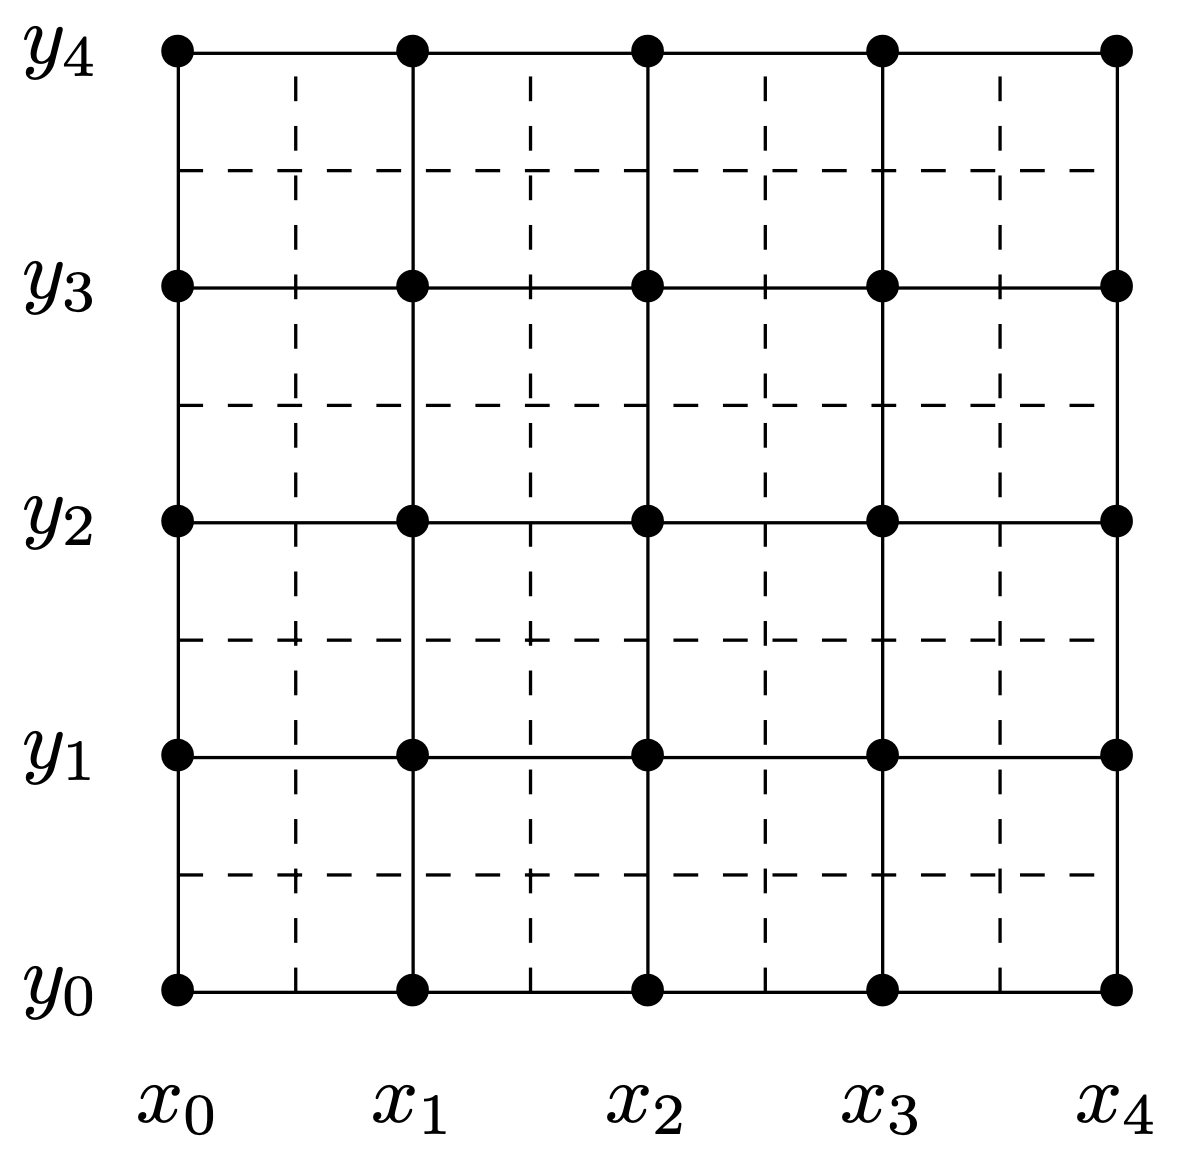
\includegraphics[width=80mm]{grids_2D.png}
\end{figure}

These degrees of freedom also characterize the {\em reduction operators} 
$\mathcal{R}_\ell$ and $\tilde{\mathcal{R}}_\ell$ mapping the continuous spaces
to the discrete ones.

They are defined as follows: 
\begin{itemize}
	\item 
	for a continuous potential $\phi$,
	the $\mathcal{C}_0$ degrees of freedom are the node values on the primal nodes:
	\begin{equation*}
		\mathcal{R}_0(\phi)_{i,j,k} := \phi(x_i,y_j,z_k)
	\end{equation*}
	and if the latter are known then the coefficients of the discrete potential may be set to
	\begin{equation*}
		\arr{\phi} = \mathcal{R}_0(\phi) \in \mathcal{C}_0.
	\end{equation*}

	\item
	for a continuous electric field $\bE$,
	the $\mathcal{C}_1$ degrees of freedom are the circulations on the primal edges:
	\begin{equation*}
		\begin{cases}
		\mathcal{R}^x_1(E_x)_{\iph,j,k} := \int_{x_i}^{x_{i+1}} E_x(x,y_j,z_k)\dd x &
		\\
		\mathcal{R}^y_1(E_y)_{i,\jph,k} := \int_{y_j}^{y_{j+1}} E_y(x_i,y,z_k)\dd y &
		\\
		\mathcal{R}^z_1(E_z)_{i,j,\kph} := \int_{z_k}^{z_{k+1}} E_z(x_i,y_j,z)\dd z &
		\end{cases}
	\end{equation*}
	and if the latter are known then the coefficients of the discrete field may be set to
	\begin{equation*}
		\arr{E} = (\arr{E}^x, \arr{E}^y, \arr{E}^z) = \mathcal{R}_1(\bE) \in \mathcal{C}_1, 
		\qquad \text{i.e.} \qquad
		\left\{\begin{aligned}
		&\arrE^x = \mathcal{R}^x_1(E_x)
		\\
		&\arrE^y = \mathcal{R}^y_1(E_y)
		\\
		&\arrE^z = \mathcal{R}^z_1(E_z)
		\end{aligned}\right.
	\end{equation*}

	\item
	for a continuous magnetic field $\bB$,
	the $\mathcal{C}_2$ degrees of freedom are the fluxes on the primal faces:
	\begin{equation*}
		\begin{cases}
		\mathcal{R}^x_2(B_x)_{i,\jph,\kph} := \int_{y_j}^{y_{j+1}}\int_{z_k}^{z_{k+1}} B_x(x_i,y,z)\dd y \dd z &
		\\
		\mathcal{R}^y_2(B_y)_{\iph,j,\kph} := \int_{x_i}^{x_{i+1}}\int_{z_k}^{z_{k+1}} B_y(x,y_j,z)\dd x \dd z &
		\\
		\mathcal{R}^z_2(B_z)_{\iph,\jph,k} := \int_{x_i}^{x_{i+1}}\int_{y_j}^{y_{j+1}} B_z(x,y,z_k)\dd x\dd y &
		\end{cases}
	\end{equation*}
	and if the latter are known then the coefficients of the discrete field may be set to
	\begin{equation*}
		\arr{B} = (\arr{B}^x, \arr{B}^y, \arr{B}^z) = \mathcal{R}_2(\bB) \in \mathcal{C}_2 ,
		\qquad \text{i.e.} \qquad
		\left\{\begin{aligned}
		&\arrB^x = \mathcal{R}^x_2(B_x)
		\\
		&\arrB^y = \mathcal{R}^y_2(B_y)
		\\
		&\arrB^z = \mathcal{R}^z_2(B_z)
		\end{aligned}\right.
	\end{equation*}
	
	\item
	for a continuous density $g$ (not used in the Gempic-Maxwell equations),
	the $\mathcal{C}_3$ degrees of freedom would be the integrals on the primal cells:
	\begin{equation*}
		\mathcal{R}_3(g)_{\iph,\jph,\kph} := \int_{x_i}^{x_{i+1}}\int_{y_j}^{y_{j+1}}\int_{z_k}^{z_{k+1}} g(x,y,z)\dd x\dd y \dd z
	\end{equation*}
	and a discrete (primal) density may be defined as
	\begin{equation*}
		\arr{g} = \mathcal{R}_3(g) \in \mathcal{C}_3.
	\end{equation*}

\end{itemize}

The primal gradient, curl and div operators, namely 
$\mat{G}: \mathcal{C}_0 \to \mathcal{C}_1$, 
$\mat{C}: \mathcal{C}_1 \to \mathcal{C}_2$ and
$\mat{D}: \mathcal{C}_2 \to \mathcal{C}_3$ 
then correspond to the incidence matrices relating nodes to edges, edges to faces 
and faces to cells (see below for more details on discrete differential operators).

On the dual grid, geometric degrees of freedom are defined similarly to the primal ones:
\begin{itemize}
	\item 
	for a continuous field $\bH$,
	the $\tilde{\mathcal{C}}_1$ degrees of freedom are the circulations on the dual edges:
	\begin{equation*}
		\begin{cases}
			\tilde{\mathcal{R}}^x_1(H_x)_{i,\jph,\kph} := \int_{x_\imh}^{x_{\iph}} H_x(x,y_\jph,z_\kph)\dd x &
			\\
			\tilde{\mathcal{R}}^y_1(H_y)_{\iph,j,\kph} := \int_{y_\jmh}^{y_{\jph}} H_y(x_\iph,y,z_\kph)\dd y &
			\\
			\tilde{\mathcal{R}}^z_1(H_z)_{\iph,\jph,k} := \int_{z_\kmh}^{z_{\kph}} H_z(x_\iph,y_\jph,z)\dd z &
		\end{cases}
	\end{equation*}
	and if the latter are known then the coefficients of the discrete field may be set to
	\begin{equation*}
		\tilde{\arr{H}} = (\tilde{\arr{H}}^x, \tilde{\arr{H}}^y, \tilde{\arr{H}}^z) = \tilde{\mathcal{R}}_1(\bH) \in \tilde{\mathcal{C}}_1
		\qquad \text{i.e.} \qquad
		\left\{\begin{aligned}
		&\tilde{\arr{H}}^x = \tilde{\mathcal{R}}^x_1(H_x)
		\\
		&\tilde{\arr{H}}^y = \tilde{\mathcal{R}}^y_1(H_y)
		\\
		&\tilde{\arr{H}}^z = \tilde{\mathcal{R}}^z_1(H_z)
		\end{aligned}\right.
	\end{equation*}	
	
	\item
	for a continuous current density $\bJ$,
	the $\tilde{\mathcal{C}}_2$ degrees of freedom are the fluxes on the dual faces:
	\begin{equation*}
		\begin{cases}
			\tilde{\mathcal{R}}^x_2(J_x)_{\iph,j,k} := \int_{y_\jmh}^{y_{\jph}} \int_{z_\kmh}^{z_{\kph}} J_x(x_\iph,y,z)\dd y \dd z &
			\\
			\tilde{\mathcal{R}}^y_2(J_y)_{i,\jph,k} := \int_{x_\imh}^{x_{\iph}} \int_{z_\kmh}^{z_{\kph}} J_y(x,y_\jph,z)\dd x \dd z &
			\\
			\tilde{\mathcal{R}}^z_2(J_z)_{i,j,\kph} := \int_{x_\imh}^{x_{\iph}} \int_{y_\jmh}^{y_{\jph}} J_z(x,y,z_\kph)\dd x \dd y &		
		\end{cases}
	\end{equation*}
	and if the latter are known then the coefficients of the discrete density may be set to
	\begin{equation*}
		\tilde{\arr{J}} = (\tilde{\arr{J}}^x, \tilde{\arr{J}}^y, \tilde{\arr{J}}^z) 
			= \tilde{\mathcal{R}}_2(\bJ) \in \tilde{\mathcal{C}}_2
		\qquad \text{i.e.} \qquad
		\left\{\begin{aligned}
			&\tilde{\arr{J}}^x = \tilde{\mathcal{R}}^x_2(J_x)
			\\
			&\tilde{\arr{J}}^y = \tilde{\mathcal{R}}^y_2(J_y)
			\\
			&\tilde{\arr{J}}^z = \tilde{\mathcal{R}}^z_2(J_z)
		\end{aligned}\right.
	\end{equation*}	
	Note: the field ${\bs D}$ is discretized using the same degrees of freedom.
	
	\item 
	Finally, for a continuous density $\rho$,
	the $\tilde{\mathcal{C}}_3$ degrees of freedom are the integrals on the dual cells:
	\begin{equation*}
		\tilde{\mathcal{R}}_3(\rho)_{i,j,k} := \int_{x_\imh}^{x_{\iph}}\int_{y_\jmh}^{y_{\jph}} \int_{z_\kmh}^{z_{\kph}} \rho(x,y,z) \dd x \dd y \dd z 
	\end{equation*}
	and the discrete density may be defined as
	\begin{equation*}
		\tilde{\arr{\rho}} = \tilde{\mathcal{R}}_3(\rho) \in \tilde{\mathcal{C}}_3.
	\end{equation*}
\end{itemize}
	
The dual differential operators, namely 
$\tilde{\mat{G}}: \mathcal{C}_0 \to \mathcal{C}_1$,
$\tilde{\mat{C}}: \mathcal{C}_1 \to \mathcal{C}_2$ and 
$\tilde{\mat{D}}: \mathcal{C}_2 \to \mathcal{C}_3$ 
then correspond to the incidence matrix on the dual grid.
With homogeneous or periodic boundary conditions these
operator matrices are the adjoint of the primal ones.

\textbf{Note}: in practice when solving the discrete Maxwell equations,
the discrete sources $\tilde{\arr{\rho}}$ and $\tilde{\arr{J}}$ are obtained by applying these 
reduction operators to the numerical particle densities represented
with smoothing splines: this will be described in Section~\ref{sec:deposition_of_part_densities}. 
(The discrete fields are then obtained by solving the discrete Maxwell equations, not by applying
the reduction operators to the unkown exact fields.)


\subsection{Some remarks on the notation for primal-dual de Rham diagrams}

% At the discrete level the general case is represented by the following diagram:

A few observations can be made about the notation used in
Diagram \ref{fig:CGL}:
\begin{itemize}
    \item This notation preserves the symmetry:
		in both complexes the discrete differential operators correspond to the strong operators of their continuous sequence, and the space numbers are intrinsic as they correspond to the degree of the differential forms.
		
		\item The Hodge operators are written with only one index corresponding to the starting space (and $\tilde{\mathbb{H}}$ if it starts from the dual complex).

		\item The diagrams should commute except for the dashed lines (i.e. the Hodge operators). In particular, the dual Hodge operators do not need to be inverse of the primal ones
		(they do not even need to be represented by square matrices).

		\item Here the spaces $\cV_\ell$ and $\tilde{\cV}_\ell$ in the continuous sequences 
		are a priori infinite-dimensional function spaces. A standard choice corresponding
		to the Hilbert-complex theoretical framework of \cite{Arnold.Falk.Winther.2010.bams}
		is to take $L^2$ spaces with $L^2$ derivatives and proper boundary conditions as 
		described below.		
		
		\item The reduction (commuting) operators 
		$\cR_\ell$ and $\tilde {\cR}_\ell$ may not be defined 
		on the full spaces $\cV_\ell$ and $\tilde{\cV}_\ell$: their domain spaces may 
		(and often do) consist of smaller spaces of smoother functions.

\end{itemize}

\subsection{Boundary conditions}
\label{sec:boundary_conditions}

In the full space $\Omega = \RR^3$ or with periodic boundary conditions,
the simplest choice is to consider 
\begin{equation} \label{eq:dR_spaces_nobound}
  \cV_0 = \tilde{\cV}_0 = H^1(\Omega), \quad
    \cV_1 = \tilde{\cV}_1 = H(\curl;\Omega), \quad
      \cV_2 = \tilde{\cV}_2 = H(\Div;\Omega), \quad
        \cV_3 = \tilde{\cV}_3 = L^2(\Omega).
\end{equation}		
In a bounded domain, boundary conditions are in general imposed
so that integration by parts hold between primal and dual spaces without boundary terms,
in the sense that
$$
\sprod{\grad \vp}{\tilde \bC} = -\sprod{\vp}{\Div \tilde \bC},
\qquad
\sprod{\curl \bF}{\tilde \bG} = \sprod{\bF}{\curl \tilde \bG},
\qquad
\sprod{\Div \bC}{\tilde \vp} = -\sprod{\bC}{\grad \tilde \vp}
$$
(with $L^2(\Omega)$ scalar products) 
should hold for all $\vp \in \cV_0$, $\bF \in \cV_1$, $\bC \in \cV_2$,
and all $\tilde \vp \in \tilde{\cV}_0$, $\tilde \bF \in \tilde{\cV}_1$,
$\tilde \bC \in \tilde{\cV}_2$.
For instance if the primal space has no boundary condition,
\begin{equation} \label{eq:dR_spaces_inhom}
	\cV_0 = H^1(\Omega), \quad
    \cV_1 = H(\curl;\Omega), \quad
      \cV_2 = H(\Div;\Omega), \quad
        \cV_3 = L^2(\Omega).
\end{equation}		
then the dual one should have homogeneous conditions
\begin{equation} \label{eq:dR_spaces_hom}
	\tilde{\cV}_0 = H^1_0(\Omega), \quad
    \tilde{\cV}_1 = H_0(\curl;\Omega), \quad
      \tilde{\cV}_2 = H_0(\Div;\Omega), \quad
        \tilde{\cV}_3 = L^2(\Omega).
\end{equation}		
By symmetry, the opposite choice is also valid.


\subsection{Alternate notation for subordinated dual complexes}

In many cases (e.g. standard finite elements or finite differences on staggered grids), the discrete dual complex is completely determined from the primal one and in particular the dual differential operators are represented my matrices which satisfy
\begin{equation} \label{eq:diff_T}
	\tilde{\mathbb{G}} = -\mathbb{D}^\top
	\qquad 
	\tilde{\mathbb{C}} = \mathbb{C}^\top
	\qquad
	\tilde{\mathbb{D}} = -\mathbb{G}^\top
\end{equation}
which implies that the dual discrete spaces $\tilde{\mathcal{C}}_\ell$ have the same dimension as $\mathcal{C}_{3-\ell}$
(for all $\ell$). 
(In finite elements this follows from the fact that the dual discrete spaces coincide with the 
primal ones, $\tilde{V}_\ell = V_{3-\ell}$, and that the dual differentials are defined by discrete duality.)

In this case {\em a natural notation is to label the dual spaces with the indices of their primal counterparts}.
This results in the following diagram.

\begin{figure}[h]
	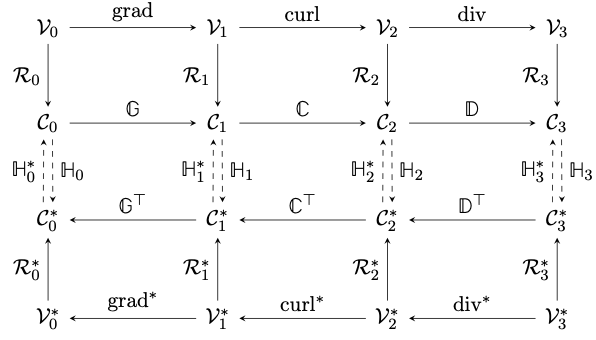
\includegraphics[width=150mm]{deRhamCGL2.png}
	\caption{Alternate notation 3D de Rham diagram}% captions are necessary for references to work
	\label{fig:CGL2}
\end{figure}	

Here the dual differential operators at the continuous level 
are {\em explicitely defined} as the adjoints of the primal ones,
and the spaces $\cV^*_\ell$ as their {\em domain spaces},
see e.g. \cite[Section~2.6]{Brezis.2011.fa}.
With the choices described in Section~\ref{sec:boundary_conditions} this yields
\begin{equation} \label{eq:diffadj}
{\grad}^* = -\Div : \cV_3^* \to \cV_2^*
\qquad 
{\curl}^* = \curl : \cV_2^* \to \cV_1^*
\qquad
{\Div}^* = -\grad : \cV_1^* \to \cV_0^*
\end{equation}
with domain spaces given by 
\begin{equation} \label{eq:cV*}
	\cV_\ell^* = \tilde{\cV}_{3-\ell}.
\end{equation}

In particular, this diagram is just another representation of the general diagram \ref{fig:CGL} 
(if it holds, i.e. if the dual sequence is subordinated to the primal one),
using the relations~\eqref{eq:diffadj}--\eqref{eq:cV*} for the continuous differential operators
and \eqref{eq:diff_T} for the discrete ones. The discrete spaces and reduction resp. Hodge 
operators then coincide,
\begin{equation}
\tilde{\mathcal{C}_\ell} = \mathcal{C}_{3-\ell}^*
\qquad 
\tilde{\mathcal{R}_\ell} = \mathcal{R}_{3-\ell}^*
\qquad 
\tilde{\mathbb{H}_\ell} = \mathbb{H}_{3-\ell}^*
\end{equation}
	

\paragraph{Illustration with Maxwell's equations}

Above the discrete Maxwell equations \eqref{eq:max_mat} 
have been written using the symmetric primal/dual notation convention.

If the diagram \ref{fig:CGL2} can be used, the discrete Maxwell's equations become
\begin{equation} \label{eq:max2}
	\left\{\begin{aligned}
		&\partial_t \arr{D}^* - \mathbb{C}^\top \arr{H}^* = - \arr{J}^*
		\\
		&\partial_t \arr{B} + \mathbb{C} \arr{E} = 0
	\end{aligned}\right.
	\quad \text{with} \quad
	\left\{\begin{aligned}
		&\arr{H}^* = \mathbb{H}_2 \arr{B}
		\\
		&\arr{E} = \mathbb{H}^*_1 \arr{D}^*
	\end{aligned}\right.
\end{equation}
with discrete unkowns (vector of coefficients) 
$$
\arr{E} \in \mathcal{C}_1, 
\quad
\arr{B} \in \mathcal{C}_2, 
\quad
\arr{H}^* \in \mathcal{C}_2^*, 
\quad
\arr{D}^* \in \mathcal{C}_1^*,
$$
and a discrete source 
\begin{equation} \label{eq:arrJ2}
	\arr{J}^* \approx \mathcal{R}_1^* {\bs J} \quad \in \mathcal{C}_1^*.
\end{equation}
Now we the indices are dictated by the primal variables (here both 
electric fields belong to ``1 spaces'' and both magnetic fields 
to ``2 spaces'', but again this could be reversed if the \Ampere{} equation
was discretized in the primal sequence).
Moreover the stability of the (source-free) equation is easily studied,
writing
$$
(\partial_t)^2 \arrE = \mathbb{H}^*_1 \mathbb{C}^\top \mathbb{H}_2 \mathbb{C} \arrE 
$$
and observing that the evolution matrix is antisymmetric as long as the (square) Hodge matrices are symmetric positive definite.

\paragraph{Illustration with Hodge Laplace's equations}

Another example is a Hodge Laplace problem of the form
\begin{equation} \label{eq:HL_cont}
		-\grad \Div \bE + \curl \curl {\bE} = {\bs F}
\end{equation}
for which a discrete version written with the diagram \ref{fig:CGL} reads
\begin{equation} \label{eq:HL}
	-\matG \t \matH_3 \t\matD \matH_1 \arrE + \t \matH_2 \t \matC \matH_2 \matC \arrE 
		= \arr{F}
\end{equation}
with $\arr{E}, \arr{F} \in \mathcal{C}_1$.
Note that neither the symmetry nor the sign of \eqref{eq:HL} are obvious.

If the dual complex can be expressed as in \ref{fig:CGL2}, the discrete equation 
takes the form
\begin{equation} \label{eq:HL2}
	\matG \matH^*_0 \matG^\top \matH_1 \arrE + \matH^*_1 \matC^\top \matH_2 \matC \arrE 
		= \arr{F}
\end{equation}
again with $\arr{E}, \arr{F} \in \mathcal{C}_1$.
Assuming again that the Hodge matrices are sdp, and that
$\matH^*_1 = (\matH_1)^{-1}$, the symmetry of the discrete operator
is easily seen by reformulating
\begin{equation} \label{eq:HL3}
	\big(\matH_1 \matG \matH^*_0 \matG^\top \matH_1 + \matC^\top \matH_2 \matC\big) \arrE 
		= \arr{F}^*
\end{equation}
with $\arr{F}^* = \matH_1 \arr{F}$.

\bibliographystyle{plainnat}
\bibliography{spectral_gempic}



\end{document}
